% Doc class required by class assignment.
\documentclass{sig-alternate-05-2015}
\usepackage{graphicx}
% copyright and other misc things provided by template.
% DOI
\doi{10.475/123_4}

% ISBN
\isbn{123-4567-24-567/08/06}

% Conference
\conferenceinfo{PLDI '13}{June 16--19, 2013, Seattle, WA, USA}

\acmPrice{\$15.00}
% end copyright
\begin{document}

% Paper title
\title{WolfTutor
  % \titlenote{(Paper 1). For use with
  % SIG-ALTERNATE.CLS. Supported by ACM.}
}
\subtitle{A system to enable peer tutoring built on Slack
  % \titlenote{A full version of this paper is available as
  % \textit{Author's Guide to Preparing ACM SIG Proceedings Using
  % \LaTeX$2_\epsilon$\ and BibTeX} at
  % \texttt{www.acm.org/eaddress.htm}
  % }
}

\numberofauthors{4} %  in this sample file, there are a *total*
\author{
  \alignauthor
  {Monica Metro}\\
  \affaddr{North Carolina State University}\\
  \affaddr{3021 F Dorner Circle}\\
  \affaddr{Raleigh, NC}\\
  \email{mgmetro@ncsu.edu}
  % 2nd. author
  \alignauthor
  {Zachery DeLong}\\
  \affaddr{North Carolina State University}\\
  \affaddr{2305 Horizon Hike Ct}\\
  \affaddr{Raleigh, NC}\\
  \email{zpdelong@ncsu.edu }
  % 3rd. author
  \alignauthor 
  {Zhangqi Zha} \\
  \affaddr{North Carolina State University}\\
  \affaddr{1800 Vienna Wood Dr}\\
  \affaddr{Raleigh, NC}\\
  \email{zzha@ncsu.edu}
}
% Generate page header.
\maketitle

% Paper body
\begin{abstract}
In this abstract, we need to preview our experiment and our results 
\end{abstract}
%%% Local Variables:
%%% mode: latex
%%% TeX-master: "../main"
%%% End:


\section{Introduction}
\label{sec:intro}
\subsection{What is WolfTutor}
\label{sec:what-wolftutor}

\subsection{WolfTutor Use Cases}
\label{sec:wolftutor-use-cases}

\subsection{Pain Points with Wolf Tutor}
\label{sec:pain-points-with}

\subsection{Initial Study}
\label{sec:initial-study}

%%% Local Variables:
%%% mode: latex
%%% TeX-master: "../../main"
%%% End:


\section{Enhancements}
\label{sec:enhancements}

\section{Architecture}
\label{sec:architecture}
% \subsection{Original Architecture}
\label{sec:Original-Architecture}
This section outlines the various components of the system and how they interact with one and another. The detailed architecture is described in figure \ref{sec:architecture:fig:O-Architecture}.

\begin{figure*}[ht]
\label{sec:architecture:fig:O-Architecture}
\caption{Original Architecture Design}
\centering
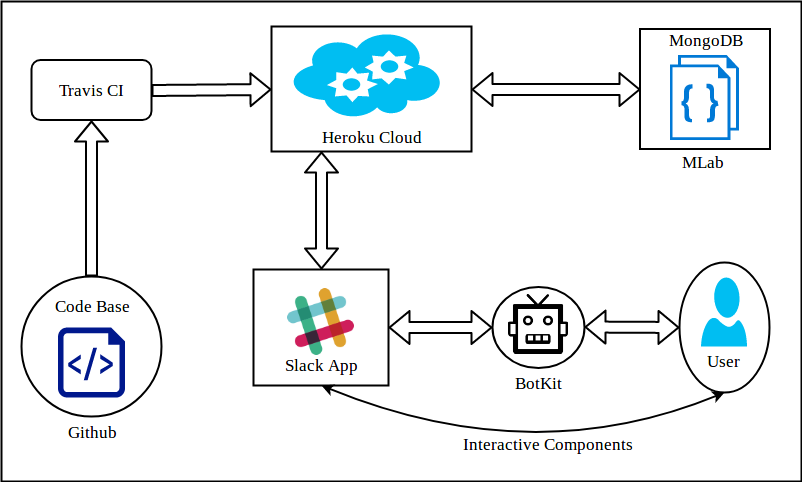
\includegraphics[width=\textwidth]{O-Architecture.png}
\end{figure*}

Broadly speaking, the architecture is divided in three main components: the slack app, the heroku cloud and the mongoDB database. This separation of concerns is a major advantage since database is independently hosted on mlab server and can be accessed from anywhere with valid authorization credentials. The heroku cloud hosts the logic of the slack app, which communicates with the user. The system also implemented the continuous deployment, continuous integration pipeline with Travis CI, which directly pushes the code to heroku cloud once the build passes (also indicated in the readme section of the repository). The test cases was also generated which acts as a sanity check for any commit made to the master branch, before deployment so as to not push broken code on the production server at heroku. Following is the detailed description of each component of the architecture.

\paragraph{Slack App}
Slack App is generated in api.slack.com dashboard. It is currently developed only for one workspace and it is configured to communicate to the heroku server which is hosted at wolftutor.herokuapp.com. Also creating a slack app gives us various authentication tokens like access token and verification token which are required for Slack to authorize that the requests and responses are coming from a valid production server. Slack app also gives us configuration of the bot like its name its icon, etc. This will be visible to the user when the user interacts with the bot. Slack bot is a part of the slack app, where bot is considered like a user (bot-user) in slack terminology. Slack app also allows access to interactive components like dialogs and message menus for the overall user experience to be more rich and interesting.

\paragraph{BotKit}
Botkit is an external library that integrates with Realtime API which can detect patterns in the user queries. The logic to be executed when a particular pattern is detected is written in the slack app (NodeJS code hosted on heroku). For instance, on saying hi user should be given an option to enroll in the system. This is one example of working of the Botkit module.

\paragraph{Code Base}
Code base is the Github repository where we maintain our code. Following the general convention, we made new branch for every new logical feature and also linked issues with particular merge commits. All this activity can be viewed in our repository. We have also used conventional practises of separating database queries and put them all together in model directory. Also all of our interactive components are in distributed in different folders.

\paragraph{Continuous Integration Module}
The master branch of our repository is linked with Travis CI to be pushed to heroku server if the build on travis CI passes. The tests written in mocha acts as a final sanity check before deploying the code on the production server. Any code that is pushed on the master is directly built on Travis CI and deployed on heroku server if build passes.

\paragraph{Heroku Server}
Heroku server is the home of our NodeJS application. We have used single dyno (free version) to host the application. The code pushed on master is deployed here by Travis and we always have the latest code in the production server. Also we have included the Procfile where it is indicated what command to execute to run the application (npm start). This is necessary for heroku to understand the starting point of the application.

\paragraph{Database}
Mlab is a server that hosts our Mongo Database. The advantage of having a remote server for mlab is that everyone can access the same data at simultaneously. In mongo, only a mongo URI is required for accessing the database along with valid user credentials. This makes it very simple to test the application locally as well as run in on the server.

\paragraph{User}
User is anyone who is signed in into the Slack workspace where the slack app is added. He/She can communicate with the app in variety of ways as described in the use-cases section. Also he/she can interact with the app using dialogs and message drop-downs and buttons to give a particular command. See details in use-cases section.

% \paragraph{
%%% Local Variables:
%%% mode: latex
%%% TeX-master: "../../../main"
%%% End:



%%% Local Variables:
%%% mode: latex
%%% TeX-master: "../../main"
%%% End:


\section{Progress}
\label{sec:progress}
% Based on the experience of previous project, the team chose the spiral model
of software development methodologies. A spiral model is a form of 
risk-driven development where the most risky parts of a project are 
identified early and planned into prototypes that can inform the final 
product. See the breakdown of the prototypes the team chose in table \ref{sec:progress:prototypes-table}.

\begin{table*}[!htbp]
\caption{Prototypes and Schedules}
\label{sec:progress:prototypes-table}
\begin{center}
\begin{tabular}{  l  l p{10cm} }
	\bf Schedules & \bf Prototypes/Work & \bf Descriptions\\ \hline \\
	Week 1 & Planning and Pre-survey & Get the original project to work, plan a few changes and enhacenments, do a user survey\\
	Week 2 & Project Proposal & Detail the plan and get ready the project proposal\\
	Week 3-1 & Prototype 1 & Gernerate dummy data, build loading history interface\\
	Week 3-2 & Prototype 2 & Gernerate dummy data, build suggestion interface\\
	Week 4-1 & Prototype 3 & Build suggestion algorithm and intergated into final system \\
	Week 4-2 & Prototype 4 & System evaluation, user testing, update system \\
	Week 5 & Presentation & Present the final system \\
	Week 6/7 & Final Paper & Draft and finalize the paper \\
\end{tabular}
\end{center}
\end{table*}


This afforded the team the ability to have regular check-ins and to measure
progress against the prototypes. The team will convene two to three times 
a week to do pair programming and to check progress against the prototypes.
When combined with regular check-ins with the TAs, the team shall be able 
to build prototype programs to perform design feature and functionality.

We also used Gitup project boards to create and track our progress. This 
method featured the ability to send a notification to the team member to 
remind and collaborate within the team members. Here is the example image.

\begin{table}[ht]
\caption{Progress Tracking Board}
\label{section:progress:tracking-board}
\centering
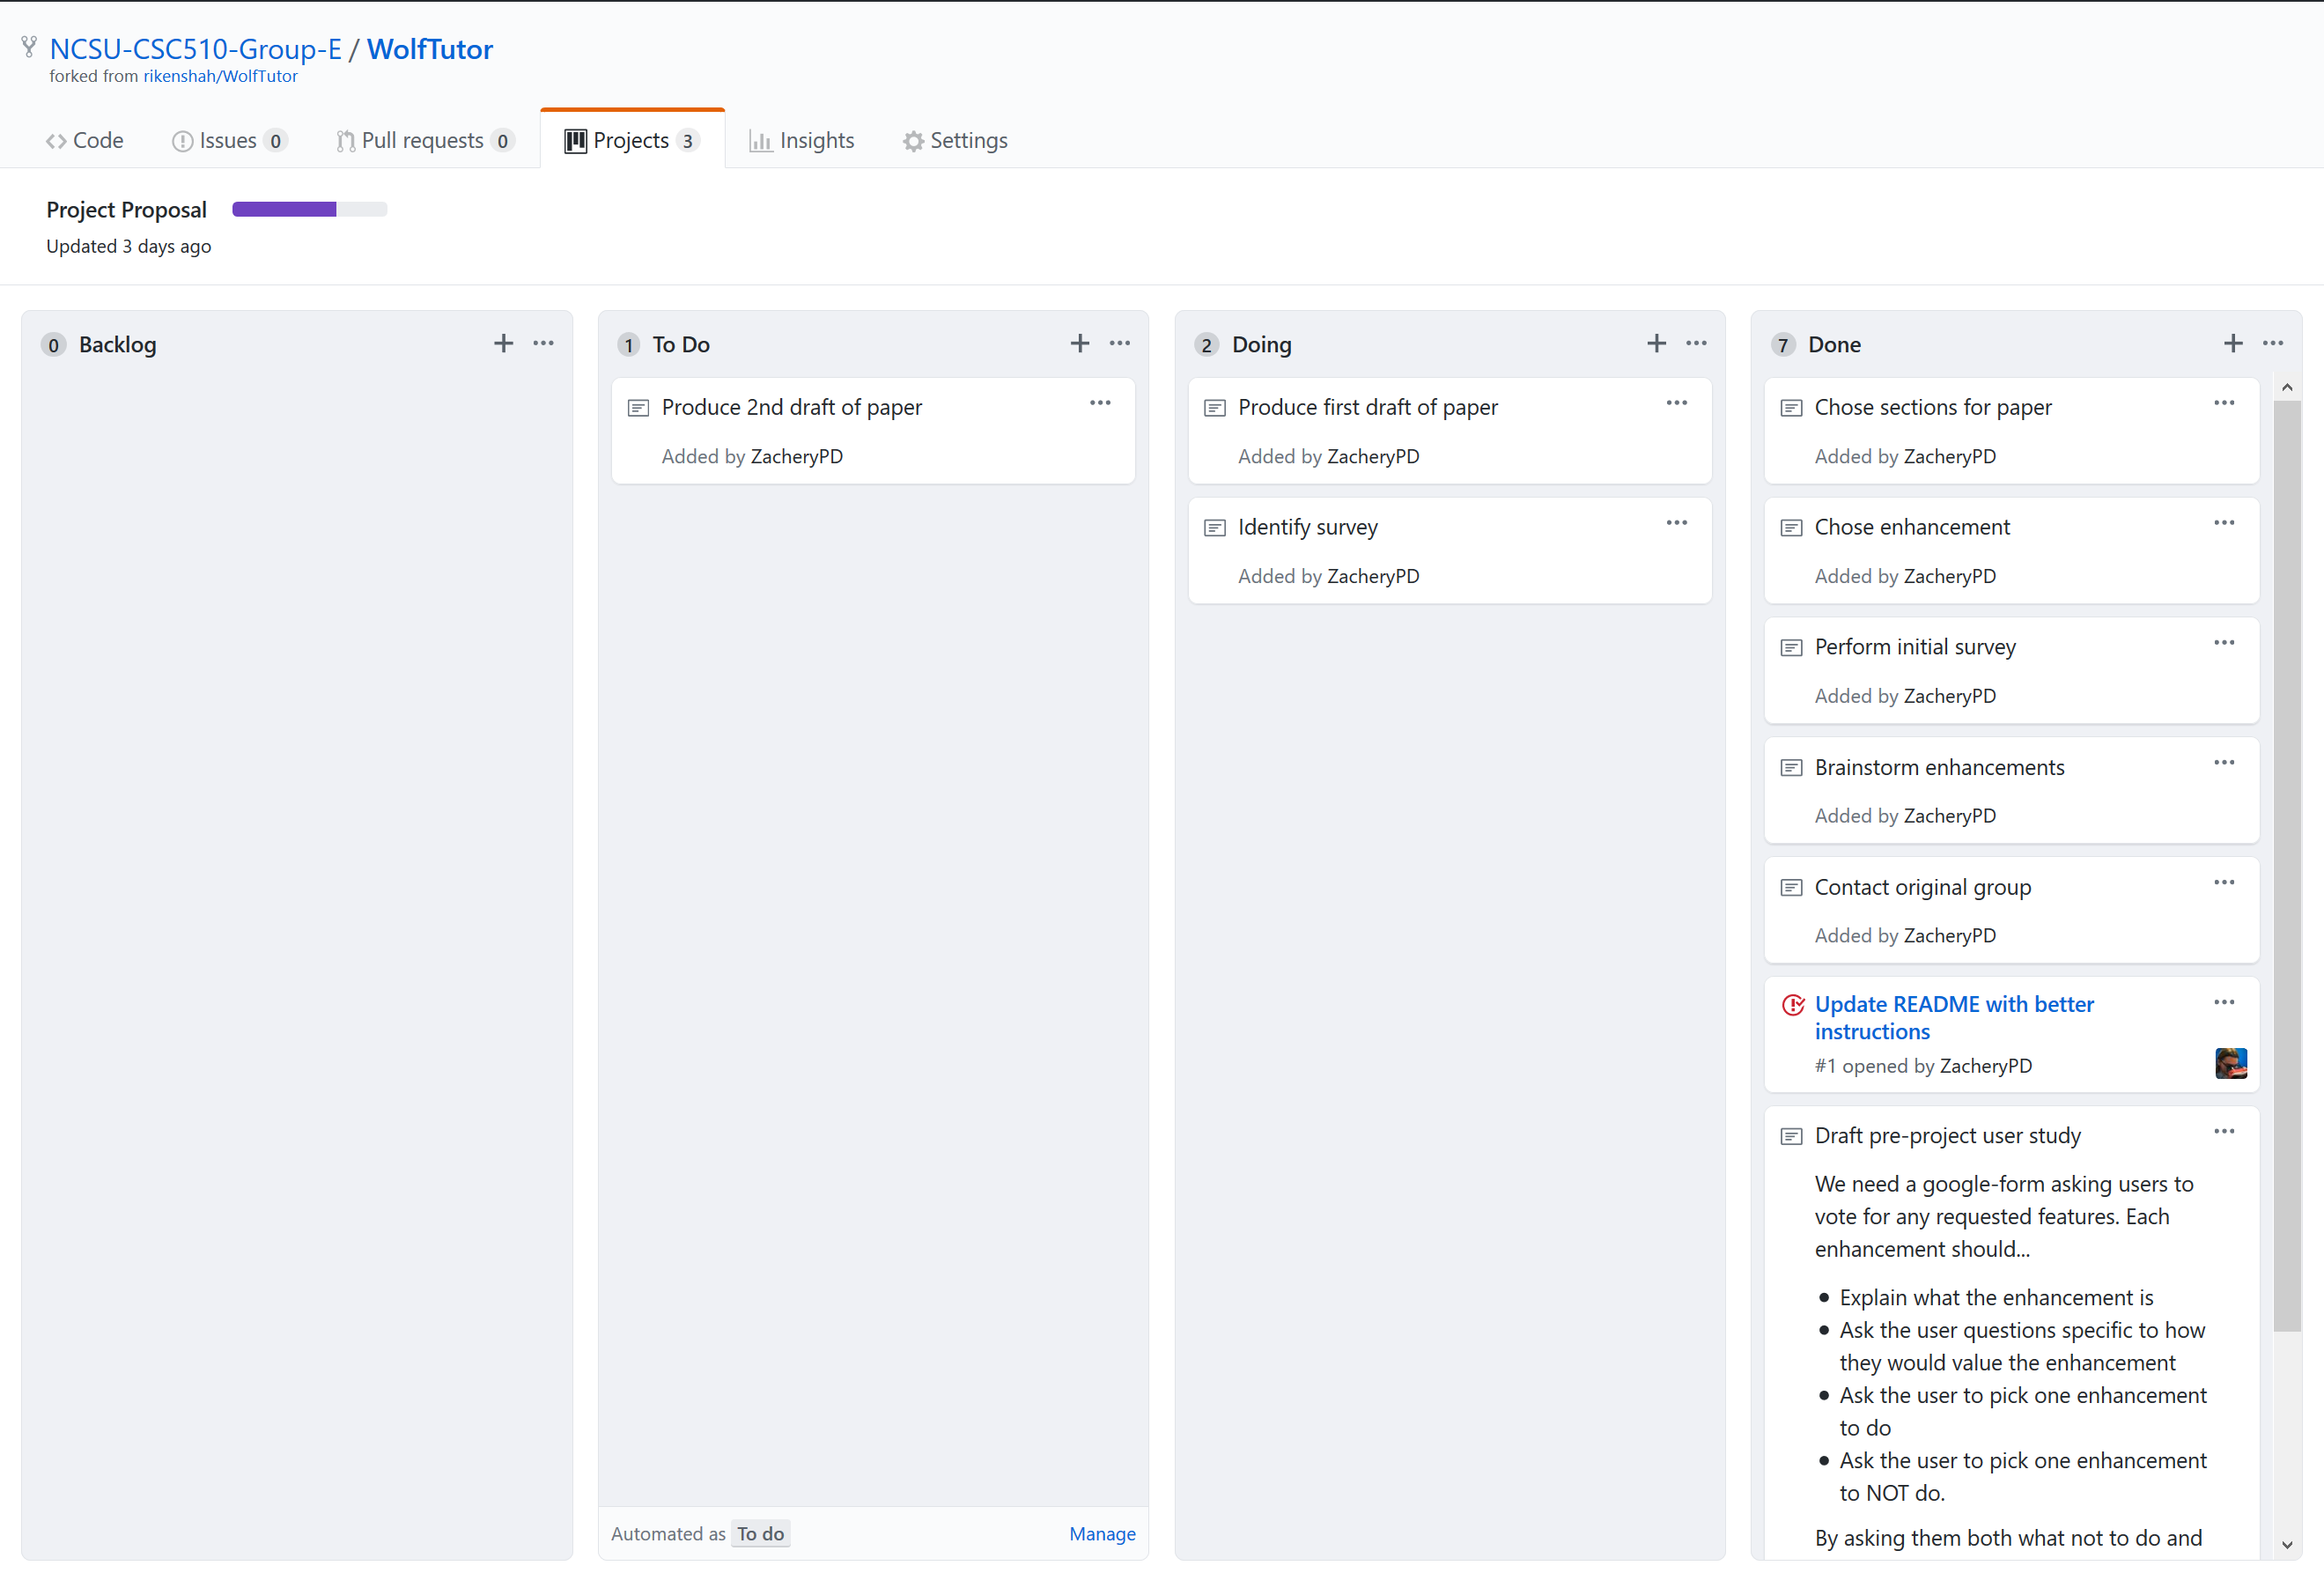
\includegraphics[width=0.48\textwidth]{progress.png}
\end{table}

\section{Validation}
\label{sec:validation}
% % What do we want to evaluate
% Why do we want to evaluate that?

\subsection{Evaluating Matching}
\label{sec:evaluating-matching}
% How?
% Process?
% Data?


\subsection{Evaluating Usability}
\label{sec:evaluating-usability}
% How
% When
% Data?


%%% Local Variables:
%%% mode: latex
%%% TeX-master: "../../main"
%%% End:


\section{Conclusion}
\label{sec:conclusion}

\subsection{Schedule}
\label{sec:schedule}
% % Please do not delete!  thanks! -- zach
% !TEX root = ../main.tex


\subsection{Future enhancement}
During our initial brainstorming and pre-survey mentioned in section \ref{sec:enhancements}, several possible enhancements were discussed. The addition of optional filters to facilitate more specific matching when searching for a tutor, integtration with commonly used online calendar applications to facilitate booking a slot and to increase ease of use, the ability to cancel or reschedule a reservaton, allowing a student to view their reservation history and to use their history to make better recommendations for their next tutor, and integrating an online video interface to conduct tutoring sessions. Considering the short time frame for the project, we chose to implement the feature that was rated as the most important by our intended audience: viewing reservation history and giving recommendations for tutors with the goal of recommending a tutor the student would rate highly. The other features will be considered as future enhancements.


% REMOVE NOCITE OR IT WILL LIST EVERYTHING IN YOUR DATABASE AS A REFERENCE
% \nocite{*}

% Bibliography/style
\bibliographystyle{abbrv}

\bibliography{export}
% End bibliography/style

\end{document}
